\documentclass[11pt]{report}
\usepackage[
  dissertation
 ,final
 ,raggedbottom
]{USCthesis}

% guidelines for manuscript formatting: http://graduateschool.usc.edu/wp-content/themes/fictional-university-theme/assets/doc/Manuscript_Formatting_and_Documentation_Styles.pdf

%% our customizations %%%%%%%%%%%%%%%%%%%%%%%%%%%%%%%%%%%%%%%%%%%%%%%%%%
\usepackage[export]{adjustbox} % for frame option in \includegraphics
\usepackage{amsmath}
\usepackage{amssymb}
\usepackage{array}
\usepackage[utf8]{inputenc} % load inputenc before csquotes
\usepackage[english]{babel}
\usepackage[
  backend     = bibtex,
  natbib      = true,
  doi         = true,
  hyperref    = true,
  citestyle   = authoryear,
  maxbibnames = 99,
  % sortlocale  = en_US,
]{biblatex}
% pkg: biblatex
\setlength\bibitemsep{0.5\baselineskip}                 % add a line between entries
\AtEveryBibitem{\iffieldundef{doi}{}{\clearfield{url}}} % if DOI, hide URL
\AtEveryBibitem{
    \clearfield{urlyear}
    \clearfield{urlmonth}
}
\DeclareFieldFormat{labelnumberwidth}{}
\addbibresource{references.bib}
\usepackage{multirow}
\usepackage{adjustbox}
\usepackage{booktabs}
\usepackage{color, colortbl}
\usepackage{csquotes}
\usepackage{efbox}
\usepackage{enumitem}
\usepackage[shortcuts]{extdash} % use `\-/' to hyphenate words/phrases that have a dash in them
\usepackage{libertine}
\usepackage[
  showframe = false,% draw a border around textwidth
  pass      = true, % force 8.5"x11" pagesize
]{geometry}
\usepackage{graphicx}
\usepackage{hyphenat}
\usepackage{ifthen}
\usepackage{lipsum}
\usepackage{multirow}
\usepackage{parnotes}
\usepackage{pdflscape} % rotate some pages in an {landscape} environment
\usepackage{pifont}
\usepackage{ragged2e}
\usepackage{seqsplit}
\usepackage{siunitx}
\usepackage{subcaption}
\usepackage{tabularx}
\usepackage{xcolor}
\usepackage{xspace}
\usepackage{float}
\usepackage{listings}
\definecolor{codegreen}{rgb}{0,0.6,0}
\definecolor{codegray}{rgb}{0.5,0.5,0.5}
\definecolor{codepurple}{rgb}{0.58,0,0.82}
\definecolor{backcolour}{rgb}{0.95,0.95,0.92}

\lstdefinestyle{mystyle}{
    backgroundcolor=\color{backcolour},   
    commentstyle=\color{codegreen},
    keywordstyle=\color{magenta},
    numberstyle=\tiny\color{codegray},
    stringstyle=\color{codepurple},
    basicstyle=\ttfamily\footnotesize,
    language=Python,
    breakatwhitespace=false,         
    breaklines=true,                 
    captionpos=b,                    
    keepspaces=true,                 
    numbers=left,                    
    numbersep=5pt,                  
    showspaces=false,                
    showstringspaces=false,
    showtabs=false,                  
    tabsize=2
}

\lstset{style=mystyle}
\usepackage{url}
\renewcommand{\baselinestretch}{1.2} 
\newcommand{\supplement}{%
  \setcounter{table}{0}
  \renewcommand{\thetable}{S\thechapter.\arabic{table}}%
  \setcounter{figure}{0}
  \renewcommand{\thefigure}{S\thechapter.\arabic{figure}}%
  \setcounter{equation}{0}
  \renewcommand{\theequation}{S\thechapter.\arabic{equation}}%
}
\usepackage{bm}
\usepackage{outlines}

\usepackage[
  breaklinks    = true,
  colorlinks    = true,
  hypertexnames = false,
  pdfpagelabels = false,
  citecolor     = {blue!80!black},
  linkcolor     = {blue!80!black},
  urlcolor      = {blue!80!black},
]{hyperref} % load hyperref as the last package

% pkg: siunitx
% some guidelines https://physics.nist.gov/cuu/Units/checklist.html
\sisetup{
  tight-spacing  = true
  ,detect-family = true
  ,detect-mode   = true
  ,binary-units  = true    % support for MB, GB, etc.
  ,range-units   = single  % "3% to 5%" -> "3 to 5%"
  ,range-phrase  = --      % "3 to 5%"  -> "3--5%"
}

% pkg: babel, hyperref
\addto\extrasenglish{%
  \renewcommand{\chapterautorefname}{Chapter}
  \renewcommand{\sectionautorefname}{Section}
  \renewcommand{\subsectionautorefname}{Section}
  \renewcommand{\subsubsectionautorefname}{Section}
}

% pkg: url
\renewcommand{\UrlFont}{\footnotesize\tt}

% our custom commands
% \renewcommand{\ttdefault}{cmtt} % use computer modern for teletype
\usepackage[scaled=0.9]{sourcecodepro}
\usepackage[symbol]{footmisc}
% \usepackage[multiple]{footmisc}

%%% draft mode / toggle commands %%%
\usepackage{etoolbox}
\newtoggle{draft}
% \settoggle{draft}{true} % change toggle for draft or final versions
\settoggle{draft}{false} % change toggle for draft or final versions

\iftoggle{draft}{
  % if 'draft' toggle is true
  \overfullrule=10pt                       % highlight overfull hboxes
}{
  % if 'draft' toggle is false
  \PassOptionsToPackage{final}{showlabels} % hide labels on figures, etc
}

% if you're including existing papers into your thesis, it helps to put
% content behind a toggle (or conditional) so you only have to maintain
% and keep consistency on one copy. see "introduction.tex".
\newtoggle{thesis}
\settoggle{thesis}{true}

\usepackage[english]{babel}
\usepackage{blindtext}

% \usepackage[inline]{showlabels}
% \renewcommand{\showlabelfont}{\sffamily \color{blue}}
% \renewcommand{\showlabelsetlabel}[1]{\efbox{\showlabelfont #1}}
%%%%%%%%%%%%%%%%%%%%%%%%%%%%%%%%%%%%%%%%%%%%%%%%%%%%%%%%%%%%%%%%%%%%%%%%

%%% front matter %%%%%%%%%%%%%%%%%%%%%%%%%%%%%%%%%%%%%%%%%%%%%%%%%%%%%%%
\begin{document}

% title should be all caps
\title{Title}

% use your full name!
% https://cs.stanford.edu/~knuth/news19.html
% "Let's celebrate everybody's full names"
\author{First Last}

% major should be all caps
\majorfield{Major}

% date should be May, August, or December (when degrees are conferred)
\submitdate{August 2021}

%%% preface %%%%%%%%%%%%%%%%%%%%%%%%%%%%%%%%%%%%%%%%%%%%%%%%%%%%%%%%%%%%
\begin{preface}
  % \prefacesection{Dedication}
  \newenvironment{mypar}[2]
  {\begin{list}{}%
    {\setlength\leftmargin{#1}
    \setlength\rightmargin{#2}}
    \item[]}
  {\end{list}}

\begin{mypar}{0.8cm}{0.8cm}
\begin{center}
    \vspace*{\fill}
    \fontsize{14}{15}\selectfont
    \emph{Dedication}
    \vspace*{\fill}
\end{center}
\end{mypar}

  \prefacesection{Acknowledgements}
  \blindtext

  {
  \hypersetup{hidelinks} % color all links black in the preface
  \tableofcontents
  \listoftables
  \listoffigures
  }

  \prefacesection{Abstract}
  \blindtext
\end{preface}

%%% introduction %%%%%%%%%%%%%%%%%%%%%%%%%%%%%%%%%%%%%%%%%%%%%%%%%%%%%%%
\chapter{Introduction} \label{ch:introduction}
\section{Background}
\blindtext

\section{Outline of the thesis}
\blindtext

\chapter{Study I with example figures, tables, and equations} \label{ch:study-i}
{\let\thefootnote\relax\footnotetext{Publication Details: Zhu, F., Emile-Geay, J., McKay, N. P., Hakim, G. J., Khider, D., Ault, T. R., Steig, E. J., Dee, S., \& Kirchner, J. (2019). Climate models can correctly simulate the continuum of global-average temperature variability. Proceedings of the National Academy of Sciences, 201809959. \url{https://doi.org/10.1073/pnas.1809959116}}}

\section{Introduction}
\blindtext

\blindtext

\blindtext

\blindtext

\blindtext

\section{Example figures}
Figure \ref{fig:01} is borrowed from \citet{zhu_climate_2019}.

\begin{figure}[htbp]
\begin{center}
    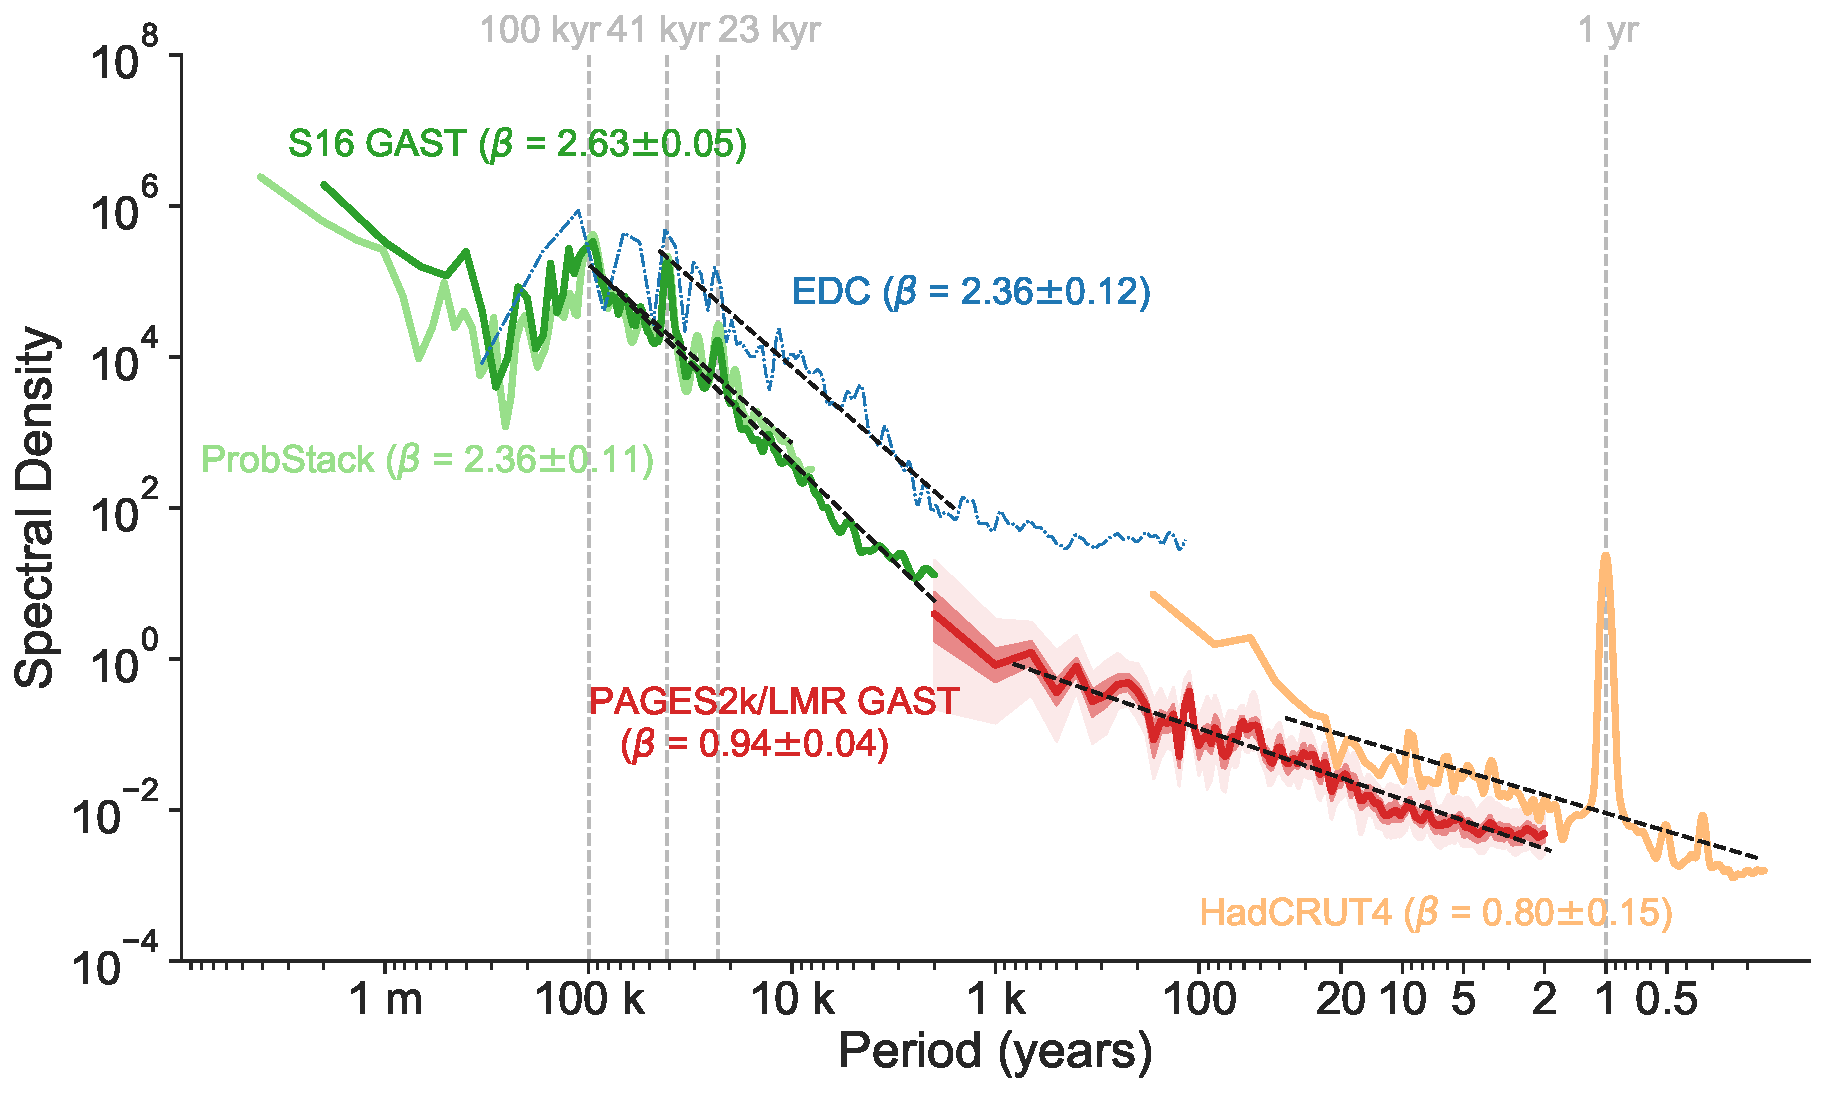
\includegraphics[width=1.0\textwidth,angle=00]{./figs/study-i-01.pdf}
    \caption{Figure borrowed from \citet{zhu_climate_2019}.}\label{fig:01}
\end{center}
\end{figure}


\section{Example tables}
Table \ref{tab:01} is an example of a simple tabular.

\begin{table}[htbp]
\centering
    \caption{Caption text.}\label{tab:01}
%     \begin{adjustbox}{width=\columnwidth,center}  % turn on if the table is too wide
    \begin{tabular}{llll}
        \toprule
        header-01 & header-02 & header-03 & header-04 \\
        \midrule
        column-01 & column-02 & column-03 & column-04 \\
    	\bottomrule
    \end{tabular}
%     \end{adjustbox}
\end{table}

\section{Example equations}
Equation \eqref{eq:01} shows a matrix.

\begin{align}
\bm{S} = \begin{bmatrix}
    \langle \bm{\Psi}_0 \mid \bm{\Psi}_0 \rangle &  \langle \bm{\Psi}_0 \mid \bm{\Psi}_1 \rangle &  \langle \bm{\Psi}_0 \mid \bm{\Psi}_2 \rangle \\
    \langle \bm{\Psi}_1 \mid \bm{\Psi}_0 \rangle &  \langle \bm{\Psi}_1 \mid \bm{\Psi}_1 \rangle &  \langle \bm{\Psi}_1 \mid \bm{\Psi}_2 \rangle \\
    \langle \bm{\Psi}_2 \mid \bm{\Psi}_0 \rangle &  \langle \bm{\Psi}_2 \mid \bm{\Psi}_1 \rangle &  \langle \bm{\Psi}_2 \mid \bm{\Psi}_2 \rangle \\
\end{bmatrix}\label{eq:01}
\end{align}

\section{Conclusion}
\blindtext

\chapter{Study II with example Python code and citations} \label{ch:study-ii}
\section{Introduction}
\blindtext

\section{Example Python code}
Below shows an example of Python code block using \texttt{Pyleoclim} \citep{pyleoclim}:
\begin{lstlisting}
import pyleoclim as pyleo

url = 'http://wiki.linked.earth/wiki/index.php/Special:WTLiPD?op=export&lipdid=MD982176.Stott.2004'
data = pyleo.Lipd(usr_path=url)
ts_list = data.to_tso()
ts_sst = pyleo.LipdSeries(ts_list)

# OUTPUT BELOW
# extracting paleoData...
# extracting: MD982176.Stott.2004
# Created time series: 6 entries
# 0 :  MD982176.Stott.2004 :  marine sediment :  depth
# 1 :  MD982176.Stott.2004 :  marine sediment :  yrbp
# 2 :  MD982176.Stott.2004 :  marine sediment :  d18og.rub
# 3 :  MD982176.Stott.2004 :  marine sediment :  d18ow-s
# 4 :  MD982176.Stott.2004 :  marine sediment :  mg/ca-g.rub
# 5 :  MD982176.Stott.2004 :  marine sediment :  sst
# 
# Enter the number of the variable you wish to use:  5
\end{lstlisting}

\section{Example citations}
Please check the ``references.bib'' file to see the details of the different types of citations.

\subsection{Journal article}
Example journal article \citet{zhu_resolving_2020}.

\subsection{Book chapter}
Example book chapter \citet{ENSObook2020:ch05}.

\subsection{Software}
Example software \citet{feng_zhu_2019_3590258}.

\section{Conclusion}
\blindtext

\chapter{Conclusion} \label{ch:conclusion}
\input{Conclusion.tex}

\addcontentsline{toc}{chapter}{Bibliography}
\begin{singlespace}
  % increase penalty such that we don't break entries over pages
  % source: https://tex.stackexchange.com/a/43275
  \patchcmd{\bibsetup}{\interlinepenalty=5000}{\interlinepenalty=10000}{}{}

  % reduce spacing between each bibentry
  \setlength\bibitemsep{0.9\baselineskip}

  % don't justify-align entries: this prevents stretching out each line
  \raggedright
  \printbibliography[title=Bibliography]
\end{singlespace}


\end{document}
